\chapter{Technical Design}\label{chap:technicaldesign}

\begin{comment}
    # Universal Design (Universal Utforming)
    # OpenLayers vs Leaflet (or others)
    # Openlayers TileWMS vs ImageWMS (optimalisering av kartet)
\end{comment}
\textcolor{orange}{
Kanskje fjerne 3.1 System arch så flytte tekst derfra hit
}

\section{System Architecture}\label{sec:systemarchitecture}

\textcolor{orange}{
Trenger noe mer tekst her kanskje, avsnitt under er flyttet fra section website. \autoref{fig:systemarchitecture}
}

The system follows a client-server architecture, where the website acts as a client and communicates with a backend server via a REST API. The processing of meteorological and geological data is handled on the server side, whereas frontend is responsible for requesting data, rendering maps, and presenting relevant information to the user.

The interaction between the website and the server is stateless, meaning that each request is independent and contains all the information needed to process it. This architectural choice improves system robustness and simplifies both development and deployment, particularly when it comes to scaling.

\begin{comment}
    I tillegg ville vi at nettsiden kun skulle snakke med med verden utenom brukeren gjennom serveren, via proxyer o.l. Dette førte til at requester gikk gjennom ett punkt, som ga en renere arkitektur. Også andre fordeler som mulighet for bedre sikkerhet, logging
\end{comment}

Using the server as an intermediary offers several advantages. While not all of these are utilized in this implementation, such an architecture allows for future expansion to include access control, credential protection for external services, and data filtering or transformation. It also simplifies integration with diverse external APIs by enabling consistent formatting before the data reaches the frontend.

\begin{figure}[h]
    \centering
    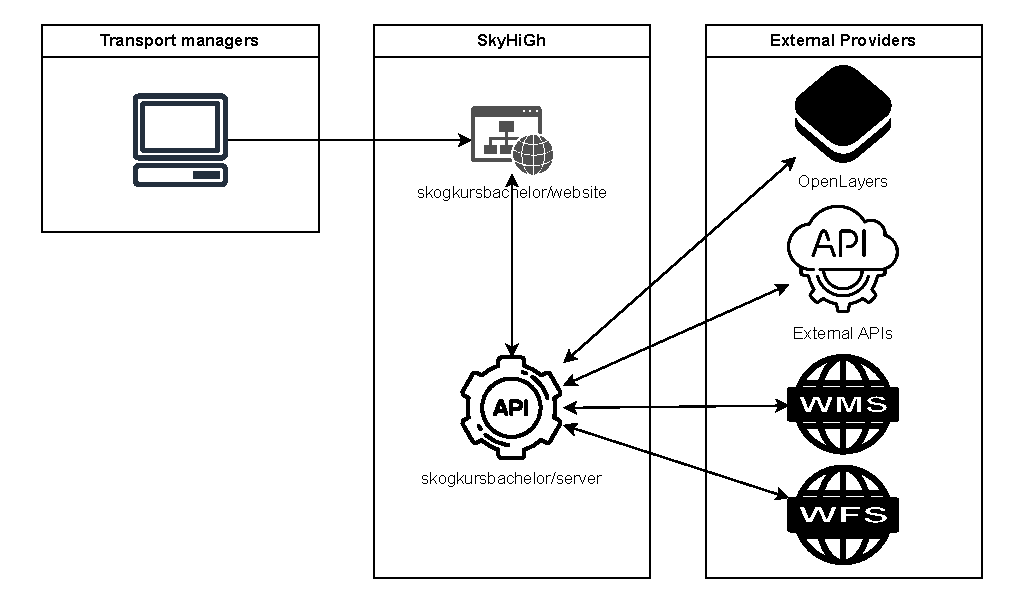
\includegraphics[width=1\linewidth]{figures/systemdesign.pdf}
    \caption{BESKRIVENDE TEKST}
    \label{fig:systemarchitecture}
\end{figure}

%\section{Data Flow} % e.g., how user requests move through the system).
%\textcolor{orange}{KANSKJE TEMP LOKASJON}

\section{Sequence Diagram}

\begin{figure}[h]
    \centering
    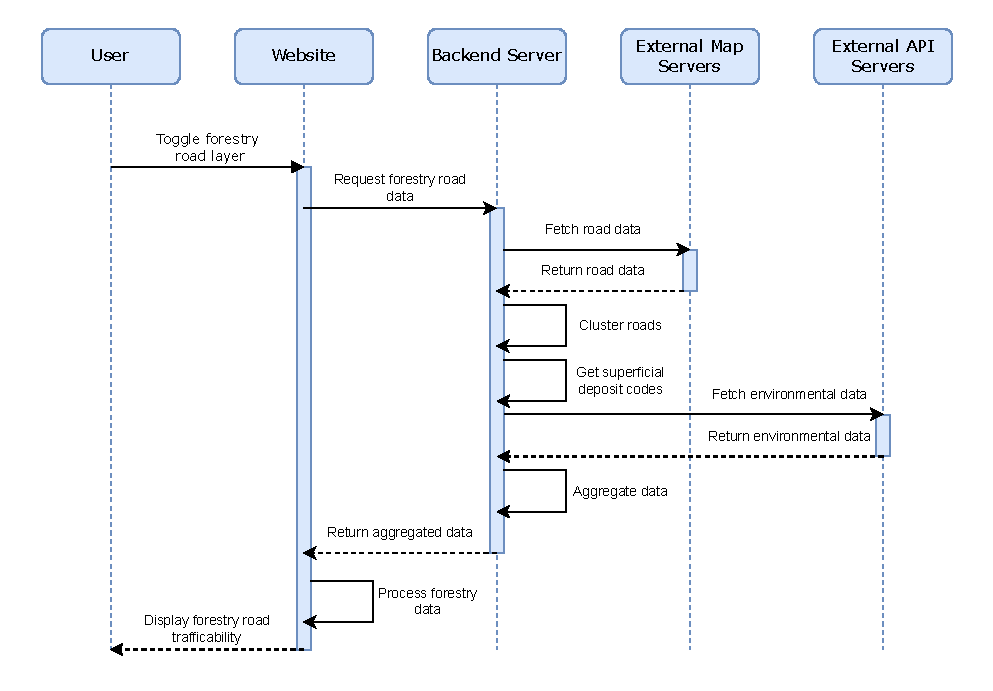
\includegraphics[width=1\linewidth]{figures/sequence_diagram.pdf}
    \caption{Sequence diagram of forestry road map layer}
    \label{fig:sequence_diagram}
\end{figure}

\autoref{fig:sequence_diagram} shows the sequence diagram for when the user toggles the forestry road map layer. The whole sequence consists of these steps:

\begin{enumerate}
    \item \textbf{Toggle forestry road layer}: The user toggles the forestry road map layer on the website.
    \item \textbf{Request forestry road data}: The website sends a request to the backend server for the necessary data within the visible map area.
    \item \textbf{Fetch road and weather data}: The backend server, acting as a proxy, fetches the required road and weather data from external map servers.
    \item \textbf{Return road and weather data}: The map servers return the requested road and weather data.
    \item \textbf{Aggregate data}: The backend server aggregates the data into a single payload.
    \item \textbf{Return aggregated data}: The backend server sends the aggregated data back to the website.
    \item \textbf{Process forestry data}: The website processes the data and determines the trafficability of roads within the visible map area.
    \item \textbf{Display forestry road trafficability}: The forestry road layer, including trafficability, is rendered on the user's map.
\end{enumerate}

\section{Website}\label{sec:technicaldesign:website}

The website serves as the user interface of the system, allowing users to visualize and interact with data related to forestry road conditions and weather-based forecasts using a dynamic map.

The classification of road trafficability is performed on the client side, as the website allows users to dynamically adjust thresholds for certain meteorological and geological parameters. A diagram detailing the classification is shown in \autoref{fig:forestryroadclassification}. Normally, this would be handled entirely by the backend server, but in order to provide immediate feedback when the user changes these thresholds, the classification logic is implemented in the frontend. This hybrid approach ensures a responsive user experience while keeping the most computationally expensive operations on the server.

\begin{figure}[h]
    \centering
    \centerline{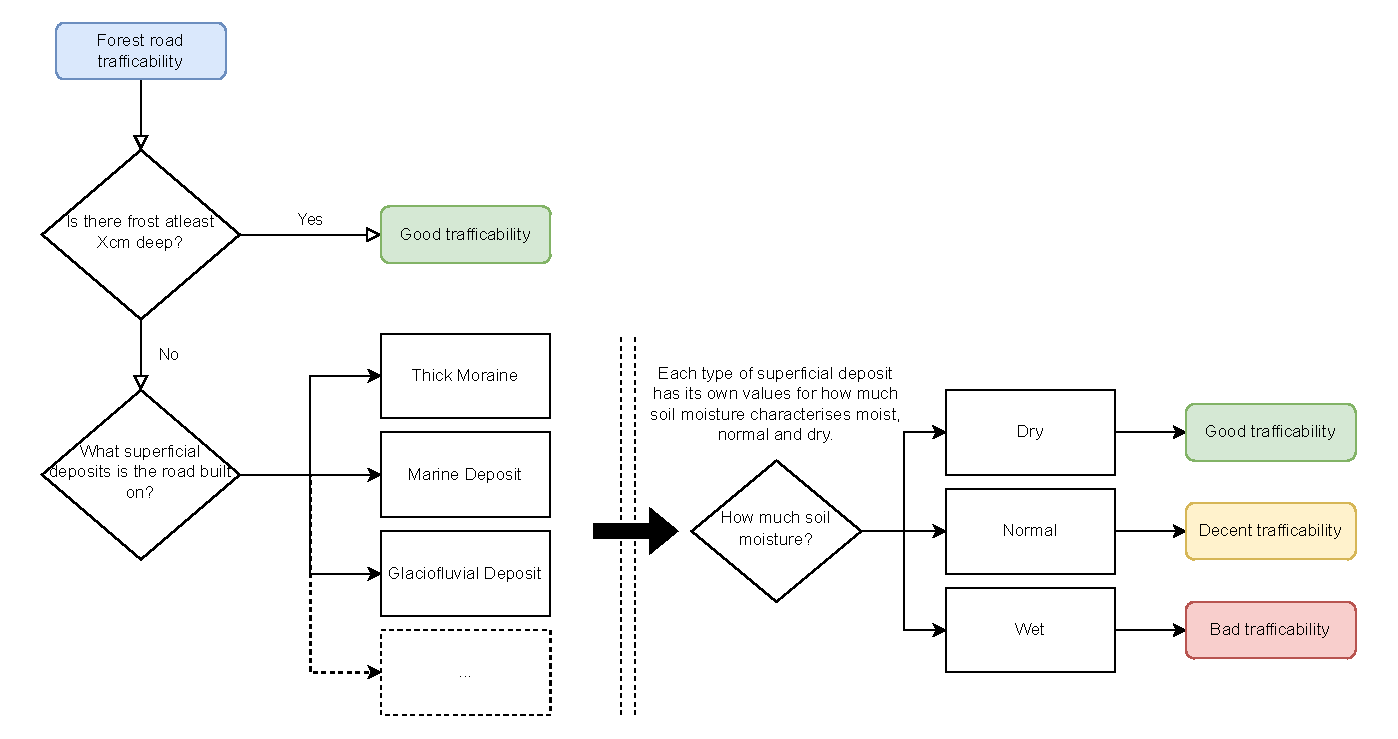
\includegraphics[width=1.2\linewidth]{figures/roadclassification.pdf}}
    \caption{Diagram visualizing the forestry road classification}
    \label{fig:forestryroadclassification}
\end{figure}

A central component of the website is its interactive map interface, which displays spatial data such as forestry road networks, map layers, and calculated trafficability classifications. The map is rendered dynamically in the browser using client-side resources, and data is loaded based on the user's current viewport and zoom level. This approach ensures efficient data usage and good performance, even when dealing with large or detailed geographic datasets.

The website is implemented as a single-page application (SPA), where all rendering and interface updates occur dynamically without full page reloads. This enables smooth interaction and better performance, as only relevant parts of the page are updated via the Document Object Model (DOM). \acrshort{html} 5 is required for full functionality, and the system relies on an active internet connection to fetch data from the server and external services. While the system is primarily intended for desktop and laptop use, it also runs on mobile devices, though the \acrshort{ui} is not optimized for smaller screens.

Choosing to implement the frontend as a web application provides several benefits. It ensures accessibility across a wide range of devices without the need for local installation, making the tool usable both in office environments and in the field.

Overall, the design of the website emphasizes a clean separation of concerns, efficiency in data handling, and accessibility, which together form a robust and user-friendly frontend component for the system.

\section{Server}

The website serves as the source of information for the website, providing map data for the website to visualize. This includes aggregation and forwarding of different map data sources, which will be discussed in \autoref{chap:mapdatasources}.


